% Created 2020-09-25 Fri 13:01
% Intended LaTeX compiler: pdflatex
\documentclass[11pt]{article}
\usepackage[utf8]{inputenc}
\usepackage[T1]{fontenc}
\usepackage{graphicx}
\usepackage{grffile}
\usepackage{longtable}
\usepackage{wrapfig}
\usepackage{rotating}
\usepackage[normalem]{ulem}
\usepackage{amsmath}
\usepackage{textcomp}
\usepackage{amssymb}
\usepackage{capt-of}
\usepackage{hyperref}
\usepackage{listings}
\IfFileExists{./resources/style.sty}{\usepackage{./resources/style}}{}
\IfFileExists{./resources/referencing.sty}{\usepackage{./resources/referencing}}{}
\addbibresource{../Resources/references.bib}
\usepackage[mode=buildnew]{standalone}
\usepackage{tikz}
\usetikzlibrary{decorations.fractals}
\usetikzlibrary{lindenmayersystems}
\author{Ryan Greenup \& James Guerra}
\date{\today}
\title{The Emergence of Patterns in Nature and Chaos Theory}
\hypersetup{
 pdfauthor={Ryan Greenup \& James Guerra},
 pdftitle={The Emergence of Patterns in Nature and Chaos Theory},
 pdfkeywords={},
 pdfsubject={},
 pdfcreator={Emacs 27.1 (Org mode 9.4)}, 
 pdflang={English}}
\begin{document}

\maketitle
\tableofcontents

\section{My Fractal}
\label{sec:org472a2d4}
My fractal really shows many unique patterns

If it is scaled by \(\varphi\) then the boxes increase two fold.

We know the dimension will be constant because the figure is self similar, so we have:

\[
\mathrm{dim} (\mathtt{my\_fractal}) = \log_{\varphi}=\frac{\log \varphi}{\log 2}
\]
\subsection{Graphics}
\label{sec:org6325d92}

\begin{figure}[htbp]
\centering
\includesvg[width=9cm]{../Problems/fractal-dimensions/scale-of-my-fractal}
\caption{\label{My-Frac-GR}TODO}
\end{figure}

\begin{figure}[htbp]
\centering
\includesvg[width=9cm]{../Problems/fractal-dimensions/my-self-rep-frac}
\caption{\label{My-Frac-GR}TODO}
\end{figure}

\begin{figure}[htbp]
\centering
\includesvg[width=9cm]{../Problems/fractal-dimensions/golden-angle-diagram}
\caption{\label{My-Frac-GR}TODO}
\end{figure}

\begin{figure}[htbp]
\centering
\includesvg[width=9cm]{../Problems/fractal-dimensions/my-self-rep-frac-ink-diagram}
\caption{\label{My-Frac-GR}TODO}
\end{figure}

\begin{figure}[htbp]
\centering
\includesvg[width=9cm]{../Problems/fractal-dimensions/My-Self-Replicating-fractal-ink}
\caption{\label{My-Frac-GR}TODO}
\end{figure}

\begin{figure}[htbp]
\centering
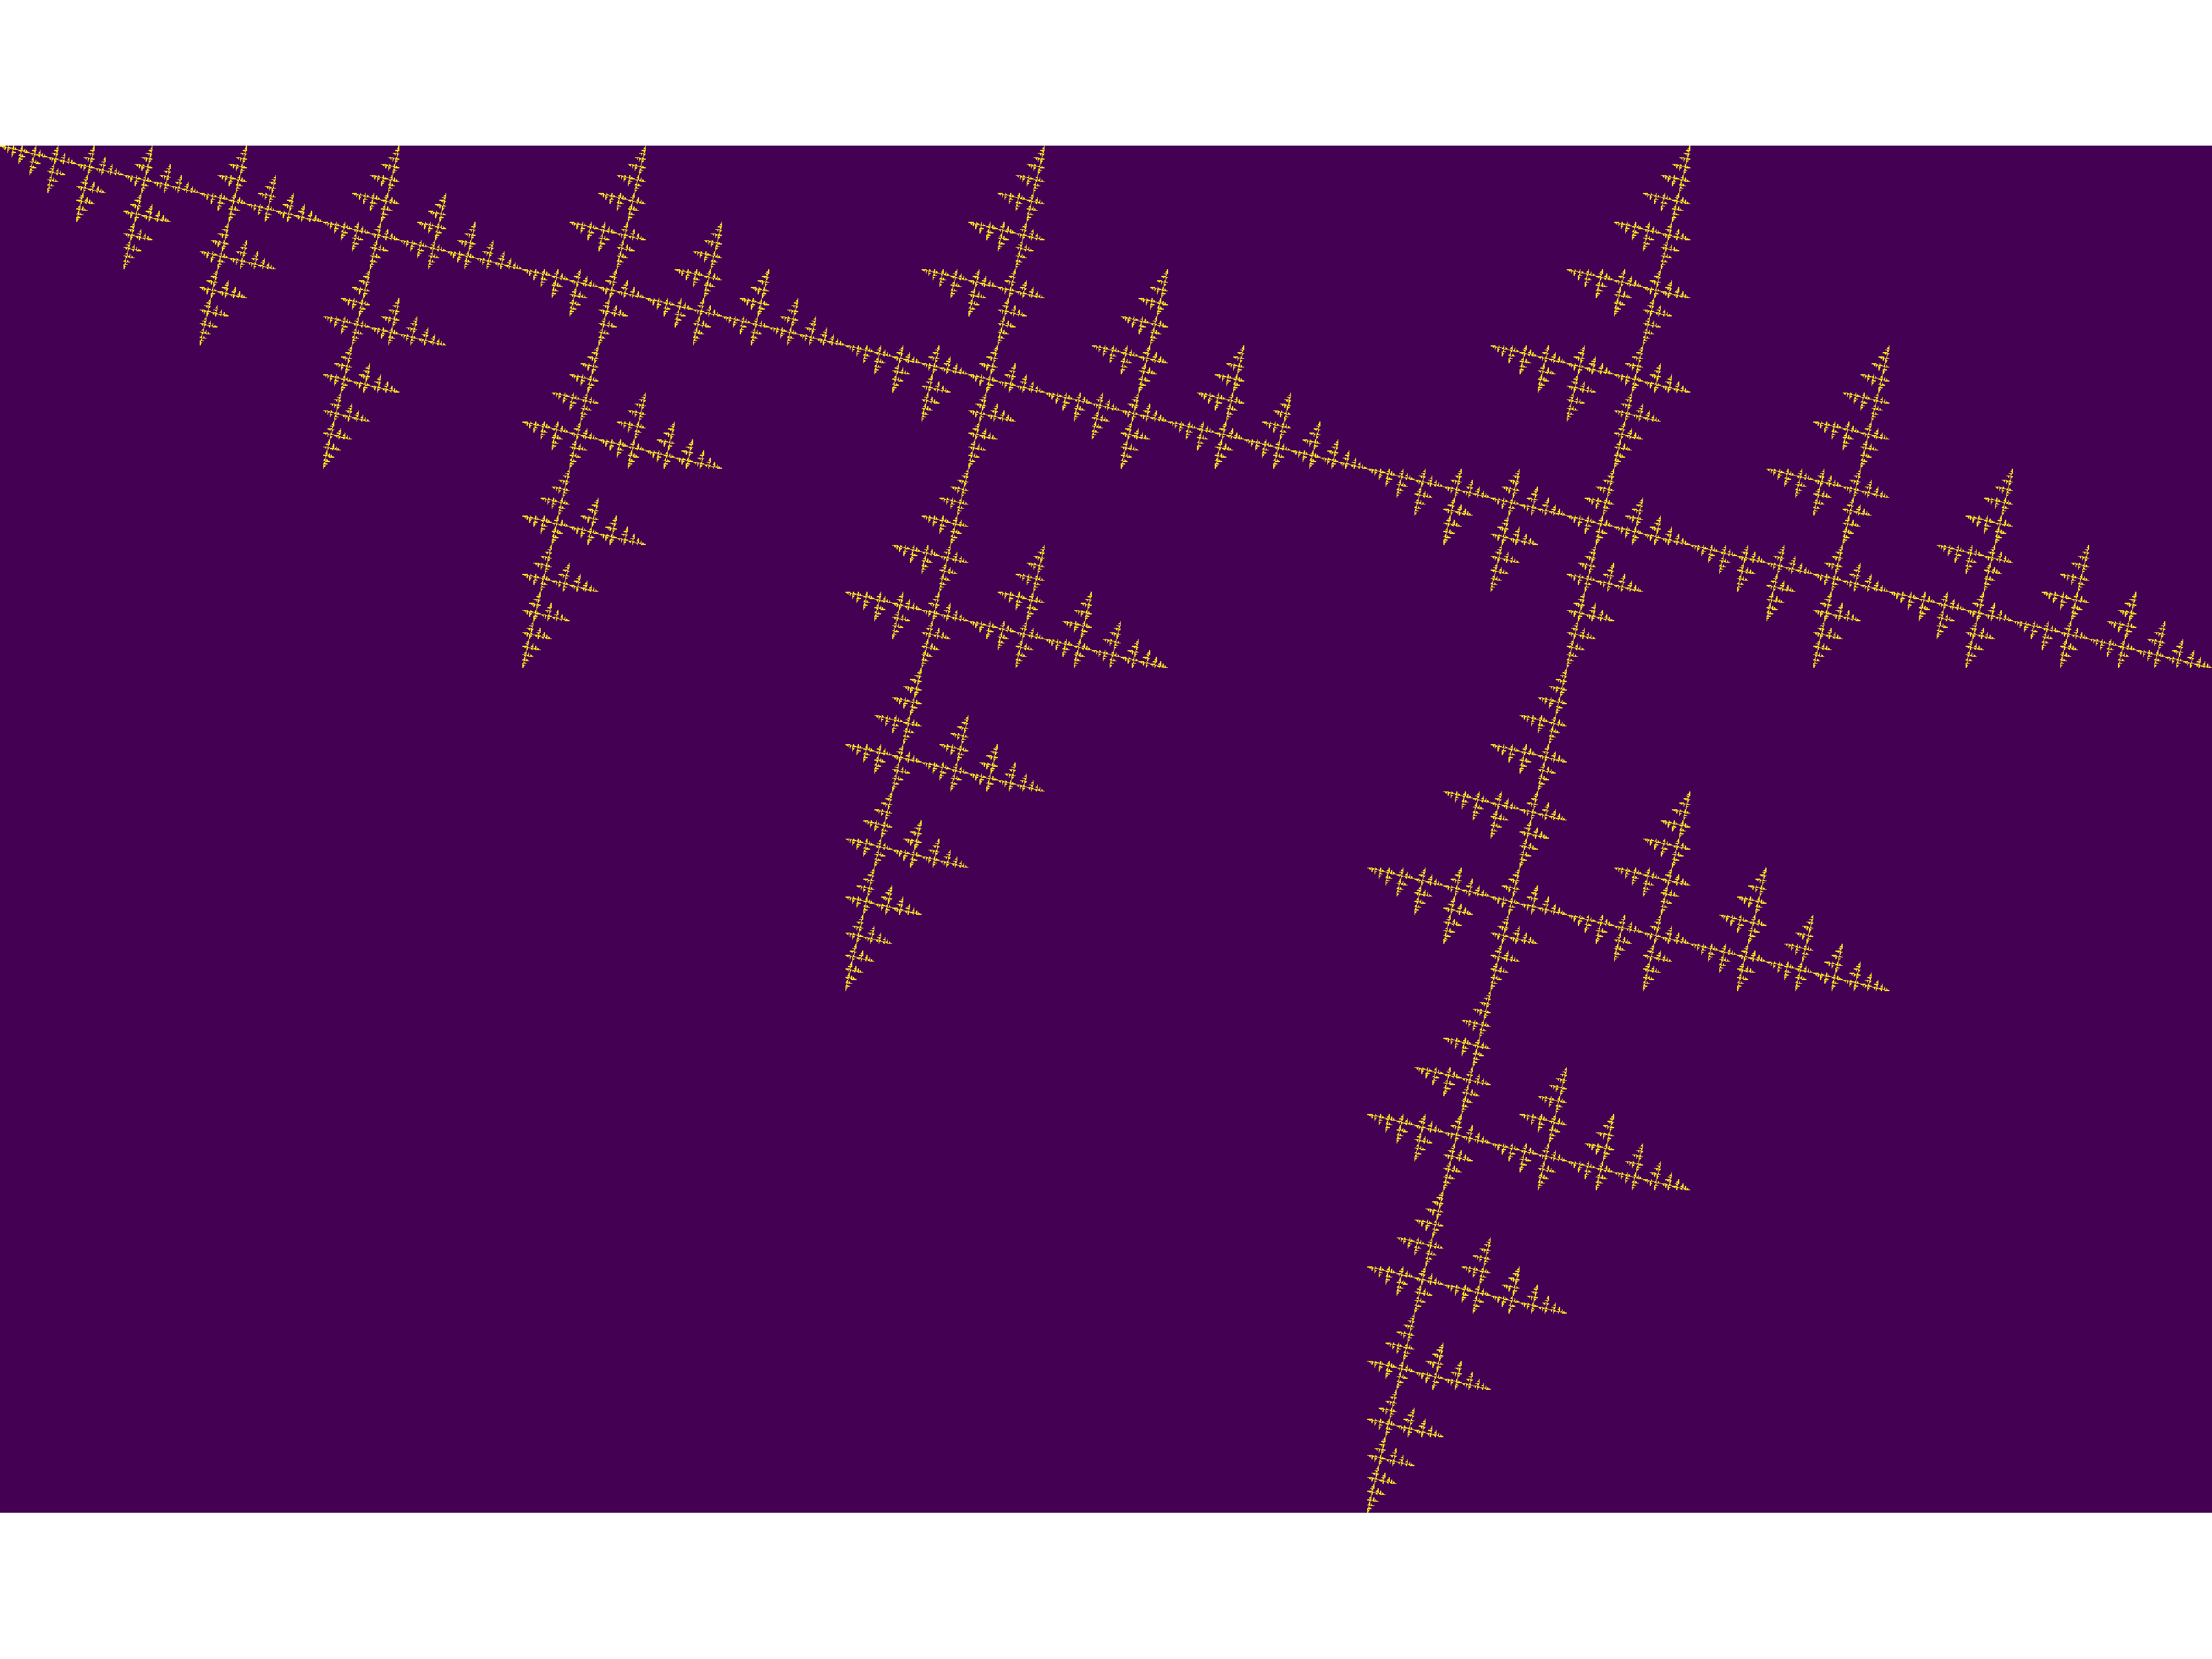
\includegraphics[width=9cm]{../Problems/fractal-dimensions/my-self-rep-frac-GR.png}
\caption{\label{My-Frac-GR}Fractal that emerges by Rotating and appending boxes, this demonstrates the relationship between the Fibonacci numbers and golden ratio very well}
\end{figure}

\begin{figure}[htbp]
\centering
\includesvg[width=9cm]{../Problems/fractal-dimensions/My-Fib-Fractal-Diagram}
\caption{\label{My-Frac-GR}Fractal that emerges by Rotating and appending boxes, this demonstrates the relationship between the Fibonacci numbers and golden ratio very well}
\end{figure}

\subsection{Discuss Pattern shows Fibonacci Numbers}
\label{sec:org7ee1a52}
\subsubsection{Angle Relates to Golden Ratio}
\label{sec:org918c6c8}
\subsection{Prove Fibonacci using Monotone Convergence Theorem}
\label{sec:orgde41de3}
Consider the series:

$$\begin{aligned}
G_n &= \frac{F_{n} }{F_{n - 1} } \\
\end{aligned}$$

Such that:

$$\begin{aligned}
F_n = F_{n- 1} +  F_{n- 2} ; \quad F_1 = F_2 = 1
\end{aligned}$$


\subsubsection{Show that the Series is Monotone}
\label{sec:orgfd6a0c2}
$$\begin{aligned}
F_{n} &> 0 \\
0 &< F_{n} \\
 \implies   0 &< F_{n - 2} +  F_{n- 1} \quad \forall n > 2 \\
  F_{n- 2} &< F_{n- 1}  \\
   \implies  F_n & < F_{n+1}
\end{aligned}$$

$$\begin{aligned}
F_{n} &> 0 \\
0 &< F_{n} \\
 \implies   0 &< F_{n - 2} +  F_{n- 1} \quad \forall n > 2 \\
  F_{n- 2} &< F_{n- 1}  \\
   \implies  F_n & < F_{n+1}
\end{aligned}$$



\subsubsection{Show that the Series is Bounded}
\label{sec:org195e118}
\subsubsection{Find the Limit}
\label{sec:org5e84884}
$$\begin{aligned}
G &= \frac{F_{n} +  F_{n+  1} }{F_{n+  1} } \\
&= 1 +  \frac{F_{n- 1} }{F_n} \\
\text{Recall that $F_n > 0 \forall n$}\\
&=  1 +  \frac{1}{    \left\lvert G \right\rvert } \\
 \implies  0 &= G^2- G +  1; \quad G > 0  \\
  \implies  G = \varphi &=  \frac{\sqrt{5} - 1  }{2} \quad  \square
\end{aligned}$$


\subsubsection{Comments}
\label{sec:org53ec531}

The Fibonacci sequence is quite unique, observe that:

This can be rearranged to show that the Fibonacci sequence is itself
when shifted in either direction, it is the sequence that does not
change during recursion.

\[\begin{aligned}
F_{n+ 1} - F_{n} = F_{n- 1} \quad \forall n > 1
\end{aligned}\]

This is analogous to how \(e^x\) doesn't change under differentiation:

$$\begin{aligned}
\frac{\mathrm{d} }{\mathrm{d} x}\left( e^x \right) \ldots
\end{aligned}$$

or how 0 is the additive identity and it shows why generating functions
are so useful.

Observe also that

$$\begin{aligned}
\lim_{n     \rightarrow \infty }\left[ \frac{F_n}{F_{n- 1} }  \right] &= \varphi \\
\lim_{n     \rightarrow \infty }\left[ \frac{F_n}{F_{n- 1} }  \right] &= \psi \\
\varphi - \psi &=  1 \\
\varphi \times  \psi  &= 1 \\
\frac{\psi}{\varphi}  = \frac{1}{\varphi^2} = \frac{1}{1-\varphi} &= \frac{1}{2-\varphi} = \frac{2}{3 - \sqrt{5}  }
\end{aligned}$$
\subsubsection{Python}
\label{sec:orge1f73ab}

\lstset{language=:exports,label= ,caption= ,captionpos=b,numbers=none}
\begin{lstlisting}
#+BEGIN_SRC python :exports both :results output graphics file :file ./a.png
#+begin_src python
import matplotlib.pyplot as plt
import sympy

plt.plot([ sympy.N(sympy.fibonacci(n+1)/sympy.fibonacci(n)) for n in range(1, 30)])
plt.savefig("./a.png")
\end{lstlisting}
\begin{center}
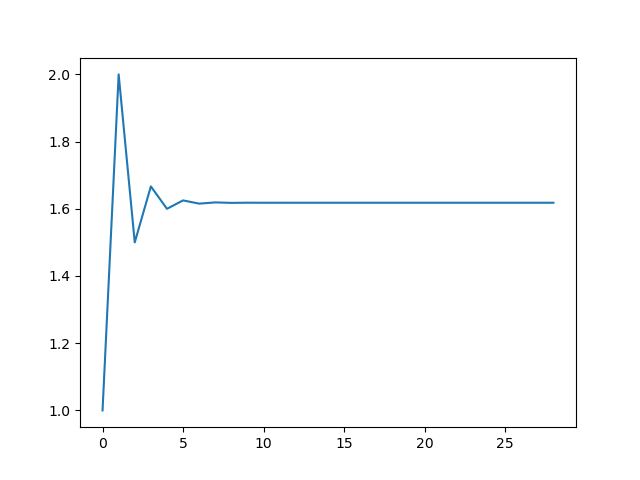
\includegraphics[width=.9\linewidth]{./a.png}
\end{center}

\subsection{Angle is \(\tan^{-1}\left( \frac{1}{1-\varphi}\right)\)}
\label{sec:orgcb2b5cb}
\subsubsection{Similar to Golden Angle \(2 \pi \left( \frac{1}{1-\varphi}\right)\)}
\label{sec:orgf2c408a}
\subsection{Dimension of my Fractal}
\label{sec:org35667a7}
\(\log_{\varphi}(2)\)
\subsection{Code should be split up or put into appendix}
\label{sec:org698a789}
\lstset{language=julia,label= ,caption= ,captionpos=b,numbers=none}
\begin{lstlisting}
function matJoin(A, B)
    function nrow(X)
        return size(X)[1]
    end
    function ncol(X)
        return size(X)[2]
    end
    emptymat = zeros(Bool, max(size(A)[1], size(B)[1]) ,sum(ncol(A) + ncol(B)) )
    emptymat[1:nrow(A), 1:ncol(A)] = A
    emptymat[1:nrow(B), (ncol(A)+1):ncol(emptymat)] = B
    return emptymat
end

function mywalk(B, n)
    for i in 1:n
        B = matJoin(B, rotl90(B));
    end
    return B
end

############################################################
##### Use Plot for themes ##################################
############################################################

using Plots
# SavePlot
## Docstring
    """
# MakePlot
Saveplot will save a plot of the fractals

- `n`
  - Is the number of iterations to produce the fractal
    - ``\\frac{n!}{k!(n - k)!} = \\binom{n}{k}``
- `filename`
  - Is the File name
- `backend`
  - either `gr()` or `pyplot()`
    - Gr is faster
    - pyplot has lines
    - Avoiding this entirely and using `GR.image()` and
     `GR.savefig` is even faster but there is no support
     for changing the colour schemes

    """
function makePlot(n, backend=pyplot())
    backend
    plt = Plots.plot(mywalk([1 1], n),
                     st=:heatmap, clim=(0,1),
                     color=:coolwarm,
                    colorbar_title="", ticks = true, legend = false, yflip = true, fmt = :svg)
    return plt
end
plt = makePlot(5)

"""
# savePlot
Saves a Plot created with `Plots.jl` to disk (regardless of backend) as both an
svg, use ImageMagick to get a PNG if necessary

- `filename`
  - Location on disk to save image
- `plt`
  - A Plot object created by using `Plot.jl`
"""
function savePlot(filename, plt)
    filename = replace(filename, " " => "_")
    path = string(filename, ".svg")
    Plots.savefig(plt, path)
    print("Image saved to ", path)
end

#------------------------------------------------------------
#-- Dimension -----------------------------------------------
#------------------------------------------------------------
# Each time it iterates the image scales by phi
# and the number of pixels increases by 2
# so log(2)/log(1.618)
# lim(F_n/F_n-1)
# but the overall dimensions of the square increases by a factor of 3
# so 3^D=5 ==> log_3(5) = log(5)/log(3) = D
using DataFrames
function returnDim()
    mat2 = mywalk(fill(1, 1, 1), 10)
    l2   = sum(mat2)
    size2 = size(mat2)[1]
    mat1 = mywalk(fill(1, 1, 1), 11)
    l1   = sum(mat1)
    size1 = size(mat1)[1]
    df = DataFrame
    df.measure = [log(l2/l1)/log(size2/size1)]
    df.actual  = [log(2)/log(1.618) ]
    return df
end

############################################################
### Main Functions ##########################################
############################################################
# Usually Main should go into a seperate .jl filename
# Then a compination of import, using, include will
# get the desired effect of top down programming.
# Combine this with using a tmp.jl and tst.jl and you're set.
# See https://stackoverflow.com/a/24935352/12843551
# http://ryansnotes.org/mediawiki/index.php/Workflow_Tips_in_Julia

# Produce and Save a Plot
#=
filename = "my-self-rep-frac";
filename = string(pwd(), "/", filename);
savePlot(filename, makePlot(5))
;convert $filename.svg $filename.png
makePlot(5, pyplot())
=#
# Return the Dimensions
returnDim()


############################################################
#### Render Image ##########################################
#################yellow and purple##########################
using GR
GR.imshow(mywalk([1 1], 5))


\end{lstlisting}
\end{document}
